% IEEE standard conference template; to be used with:
%   spconf.sty  - LaTeX style file, and
%   IEEEbib.bst - IEEE bibliography style file.
% --------------------------------------------------------------------------

\documentclass[letterpaper]{article}
\usepackage[T1]{fontenc}
\usepackage[utf8]{inputenc}
\usepackage{spconf,amsmath,amssymb,graphicx}
\usepackage[colorinlistoftodos]{todonotes}

\newcommand{\mytodo}[1]{\todo[inline]{#1}}
\newcommand{\dtodo}[1]{\todo[inline, color=cyan]{#1}}
\newcommand{\rtodo}[1]{\todo[inline, color=yellow]{#1}}
\newcommand{\ptodo}[1]{\todo[inline, nolist, color=green]{#1}}

% Example definitions.
% --------------------
% nice symbols for real and complex numbers
\newcommand{\R}[0]{\mathbb{R}}
\newcommand{\C}[0]{\mathbb{C}}

% bold paragraph titles
\newcommand{\mypar}[1]{{\bf #1.}}

% Title.
% ------
\title{Optimizing Simplex Implementation For Standard Form Problems}
%
% Single address.
% ---------------
\name{Donjan Rodic, Rico Häuselmann} 
\address{Department of Mathematics\\ ETH Zürich\\Zürich, Switzerland}

% For example:
% ------------
%\address{School\\
%		 Department\\
%		 Address}
%
% Two addresses (uncomment and modify for two-address case).
% ----------------------------------------------------------
%\twoauthors
%  {A. Author-one, B. Author-two\sthanks{Thanks to XYZ agency for funding.}}
%		 {School A-B\\
%		 Department A-B\\
%		 Address A-B}
%  {C. Author-three, D. Author-four\sthanks{The fourth author performed the work
%		 while at ...}}
%		 {School C-D\\
%		 Department C-D\\
%		 Address C-D}
%

\begin{document}
%\ninept
%
\maketitle
%

\listoftodos

\begin{abstract}
\ptodo{Describe in concise words what you do, why you do it (not necessarily
in this order), and the main result.  The abstract has to be
self-contained and readable for a person in the general area. You
should write the abstract last.}
\end{abstract}

%%%%%%%%%%%%%%%%%%%%%%%%%%%%%%%%%%%%%%%%%%%%%%%%%%%%%%%%%%%%%%%%%%%%%%%%%%%%%%%%
%%%%%%%%%%%%%%%%%%%%%%%%%%%%%%%%%%%%%%%%%%%%%%%%%%%%%%%%%%%%%%%%%%%%%%%%%%%%%%%%

\section{Introduction}\label{sec:intro}

In this section we will motivate our choice of algorithm to optimize and give
a brief overview of related work.

\mypar{Motivation} The Simplex algorithm for linear optimization is widely
used in logistics, optimizing business performance and many other fields.

The simplex solution to linear problems may be used as a crucial part in
basic decision making in business applications, for example in logistics.
In this environments performance is important. Therefore it is interesting to see how far
a solver for a specific class of linear problems can be optimized.

\mypar{Implementation} We present an implementation which is optimized 
for a limited class of linear optimization problems and solves this kind of problem
faster than any commercially available general purpose solver.

\mypar{Related work} Many production grade linear optimization packages exist.
We used three of them to compare the performance of our implementation to what is being
used in big business.
\begin{itemize}
    \item{GLPK \cite{glpk}, a free open source linear programming package.}
    \item{Gurobi \cite{gurobi}, a commercial grade package which claims to be the fastest available solution when taking into account multi-threading. Gurobi is free for educational use.}
    \item{SoPlex \cite{soplex}, free for educational use, developed at Zuse Institute Berlin (ZIB).}
\end{itemize}

%%%%%%%%%%%%%%%%%%%%%%%%%%%%%%%%%%%%%%%%%%%%%%%%%%%%%%%%%%%%%%%%%%%%%%%%%%%%%%%%
%%%%%%%%%%%%%%%%%%%%%%%%%%%%%%%%%%%%%%%%%%%%%%%%%%%%%%%%%%%%%%%%%%%%%%%%%%%%%%%%

\section{Background: The Simplex Algorithm}\label{sec:background}
It follows a brief introduction to the class of problem in consideration
and the algorithm used as well as a cost analysis of the algorithm.

\mypar{Linear Optimization Problems \cite{dantzig}}
The general formulation of a linear problem is
\begin{eqnarray*}
    \max c^T x, & \text{Subject To}\\
    b_l \leq A x \leq b_u,
\end{eqnarray*}
Where $c \in \mathbb{Q}^n$, $x \in \mathbb{R}^n$, $A \in \mathbb{Q}^{m \times n}$ and $b \in \mathbb{R}^m$.

\mypar{Standard form Linear Problems}
A linear problem is considered to be in standard form when it is formulated as
\begin{eqnarray*}
    \max c^T x, & \text{Subject To}\\
    A x \leq b \\
    x \geq 0.
\end{eqnarray*}
Any linear problem can be transformed into standard form \rtodo{citation needed?}. Considering this we chose to restrict our solver to standard form problems, since supporting other formulations would have lead to more effort being put into transforming the problem into standard form (effectively implementing a domain specific language).

\mypar{The Simplex Method}
The tableau form of the simplex method for standard form problems works as follows:
Let m be the number of constraints and n the number of variables.
\begin{enumerate}
    \item initialize the tableau $T \in \mathbb{R}^{(m+1) \times (n+m+1)}$
        \[ T = 
            \left[
            \begin{matrix}
                A & I_m & b \\
                c & 0 & 0
            \end{matrix}
            \right]
        \]
        And create a set of column indices to keep track of the currently ``active'' columns (also called the basis). 
        Initialize the basis with the indices 
        \[ B = \{ m, \dots, n+m-1 \} \]
    \item iterate:
        \begin{enumerate}
            \item (Pivoting) If $\nexists\, i\, |\, T_{m,i} < 0$ problem is solved. Else:
                \[\text{pcol} := \text{argmin}\left(T_{m,i}\right)\]
            \item (Pivoting) If $\nexists\, i\, |\, T_{i, \text{pcol}} > 0$ problem is infeasible. Else:
                (Basis Exchange)\[\text{prow} := \text{argmin}\left(\frac{T_{i, 2m}}{T_{i,\text{pcol}}} \right)\]
            \item perform Gaussian elimination:
                \[p :=  T_{\text{prow}, \text{pcol}}\]
                for $i \in \{0, \dots, m-1\}$:
                \[ T_{i,:} := T_{i,:} - T_{\text{prow},:} \frac{T_{i,\text{pcol}}}{p},\, if\, i \neq \text{prow}, \]
                and update the basis
                \[ B := B \setminus \{\text{prow}\} \cup \{\text{pcol}\}. \]
        \end{enumerate}
\end{enumerate}

\mypar{Cost Analysis}
The cost of the overall algorithm depends highly on the coefficients of the problem,
since the coefficients determine the number of iterations necessary. 
A small problem may very well take more iterations to solve than a huge one.

However, the number of operations contained in one iteration only depends on the problem size.
Let the number of iterations be $N$, then
\[ \text{\#flops} = N \times 2 m \times (m + n + 1) \]
As well as the number of doubles read from memory, which bounded from below by
\[ \frac{(m + 1) \times (m + n + 1)}{B} \leq \text{\#loads}, \]
Where $B$ is the block size of the L1 cache for very small problems where the entire
tableau fits into cache, and bounded from above by
\[ \text{\#loads} \leq N \times (3m + n) + (m + 1) \times (m + n + 1), \]
Assuming every load is a miss.

For the operational intensity this means:
\[ \frac{B\times N}{4} \leq I \leq \frac{1}{4} \]

%%%%%%%%%%%%%%%%%%%%%%%%%%%%%%%%%%%%%%%%%%%%%%%%%%%%%%%%%%%%%%%%%%%%%%%%%%%%%%%%
%%%%%%%%%%%%%%%%%%%%%%%%%%%%%%%%%%%%%%%%%%%%%%%%%%%%%%%%%%%%%%%%%%%%%%%%%%%%%%%%

\section{Our Implementation}\label{sec:yourmethod}

In this section we explain the our baseline implementation as well as all optimizations we made.
\ptodo{Now comes the ``beef'' of the paper, where you explain what you
did. Again, organize it in paragraphs with titles. As in every section
you start with a very brief overview of the section.}

\ptodo{For this class, explain all the optimizations you performed. This mean, you first very briefly
explain the baseline implementation, then go through locality and other optimizations, and finally SSE (every project will be slightly different of course). Show or mention relevant analysis or assumptions. A few examples: 1) Profiling may lead you to optimize one part first; 2) bandwidth plus data transfer analysis may show that it is memory bound; 3) it may be too hard to implement the algorithm in full generality: make assumptions and state them (e.g., we assume $n$ is divisible by 4; or, we consider only one type of input image); 4) explain how certain data accesses have poor locality. Generally, any type of analysis adds value to your work.}

\mypar{Baseline Implementation}
Our baseline implementation parses an input file containing the coefficients for the objective function and the constraints.
The coefficients are stored in a two dimensional STL vector of vector representation of the simplex tableau.

The steps performed in each iteration are separated into three functions: 
\begin{itemize}
    \item{\tt pivot\_col}
    \item{\tt pivot\_row}
    \item{\tt base\_exchange}
\end{itemize}
The first two contain the code for finding the pivot element to use in the iteration whereas
the third facilitates the Gaussian elimination step.

\mypar{Profiling}
Profiling was done with {\tt gprof}, {\tt perf} and {\tt valgrind}. All tools consistently showed that the vast majority of the
runtime is spent in the {\tt base\_exchange} function, where we focused all subsequent optimization.
Further annotated analysis revealed stalls at the memory access functions, which can be alleviated by exploiting instruction level parallelism (ILP) via static scalar assignment
where unit stride access was applicable.


\mypar{Array}
The Array optimization replaces the vector of vectors implementation of the tableau by
a C99 one dimensional contiguous array allocated and aligned using {\tt \_mm\_malloc } from
the Intel intrinsics headers.

All subsequent optimizations were based on this implementation.

\mypar{Blocking}
As a next step we added blocking in the loop that runs over the whole tableau 
inside the basis exchange. Block sizes from $1 \times 1$ to $16 \times 16$ were tried.

The code for different block sizes was generated using 
{\tt cheetah} \cite{cheetah}, a templating engine for python. The following optimizations were introduced
by changing the code templates to be able to make use of the best block size.

\mypar{Cache control}
Improvement of cache access attempted through intrinsics for non temporal assignment in order to avoid polluting the cache with updates on the active basis elements and
effective cost calculations. We further added prefetching in order to load soon-to-be-used blocks into the L2 cache, as well as prefetching parts of the current block into L1.

\mypar{Swapping}
In order to allow the compiler to perform optimization much better, the pivot and the last row
of the tableau were swapped before and after entering the main loop of the base exchange step,
allowing to get rid of the if statements used to test for the pivot row in the main loop.

This optimization does not change the number of floating point operations performed, however it affects the number of bytes loaded per iteration slightly.

\mypar{Vectorization}
In the last phase, manual vectorization using AVX instructions was performed.


\ptodo{As important as the final results is to show that you took a structured, organized approach to the optimization and that you explain why you did what you did.}

\ptodo{Mention and cite any external resources including library or other code.}

\ptodo{Good visuals or even brief code snippets to illustrate what you did are good. Pasting large amounts of code to fill the space is not good.}

%%%%%%%%%%%%%%%%%%%%%%%%%%%%%%%%%%%%%%%%%%%%%%%%%%%%%%%%%%%%%%%%%%%%%%%%%%%%%%%%
%%%%%%%%%%%%%%%%%%%%%%%%%%%%%%%%%%%%%%%%%%%%%%%%%%%%%%%%%%%%%%%%%%%%%%%%%%%%%%%%

\section{Experimental Results}\label{sec:exp}

\ptodo{Here you evaluate your work using experiments. You start again with a
very short summary of the section. The typical structure follows.}

\mypar{Experimental setup}
All experiments were conducted on a Core i5-3360M (Ivy Bridge) running GNU/Linux with 32 KB L1 cache, 256 KB L2 cache and 3 MB L3 cache, all at 64 bytes line size.

GCC 4.7.3 was used for compilation. The following flags were used:
{\tt -O3 -march\--native  } for automatic vectorization with {\tt -fno\--tree\--vectorize \\ -fno\--tree\--slp\--vectorize -mno\--abm } additionally for non vectorized code.
For profiling {\tt -g3 -ggdb -pg } was added.

A random linear problem generator was written to test the implementations. 
The problem generator is restricted for simplicity's sake to generate problems with guaranteed feasibility by allowing only positive coefficients. 
The same parameter was used for the number of Variables as well as the number of constraints.

The problem size was varied from 10 to 1000, or up to 4000 where relevant for out-of-cache comparison.
Due to the unpredictable count of steps the Simplex algorithm needs to reach a solution, each problem size was averaged over up to 100 samples.

The code was instrumentalized to count floating point and memory operations. The measured numbers for both were compared to manually computed values and found to agree.

In order to compare to third party packages, their respective API was used according to the available documentation. 
The same technique was used to measure runtime, however instrumentalization was not used.

%%%%%%%%%%%%%%%%%%%%%%%%%%%%%%%%%%%%%%%%%%%%%%%%%%%%%%%%%%%%%%%%%%%%%%%%%%%%%%%%

\mypar{Results}
\mytodo{
\mypar{Questions}
best block sizes for blocking of the elimination step?
best block sizes for unrolled/ssa calculation steps?
vectorisation useful (cf autovectorisation)?
cache control useful?
comparison to 3rd party
are we at the memory bandwidth maximum? -> roofline, yes
}


Direct comparison with alternative Simplex solvers shows that even our baseline implementation performs significantly faster.
This results from the simplicity assumptions we have made (regularity, conformity, definiteness) under which a lot of tedious checks can be eliminated.
Unfortunately none of the APIs offered to impart this information to the respective solver.
We plot the elapsed RDTSC cycles instead of per cycle performance as to not having to guess the operation count of each solver.

\begin{figure}\centering
  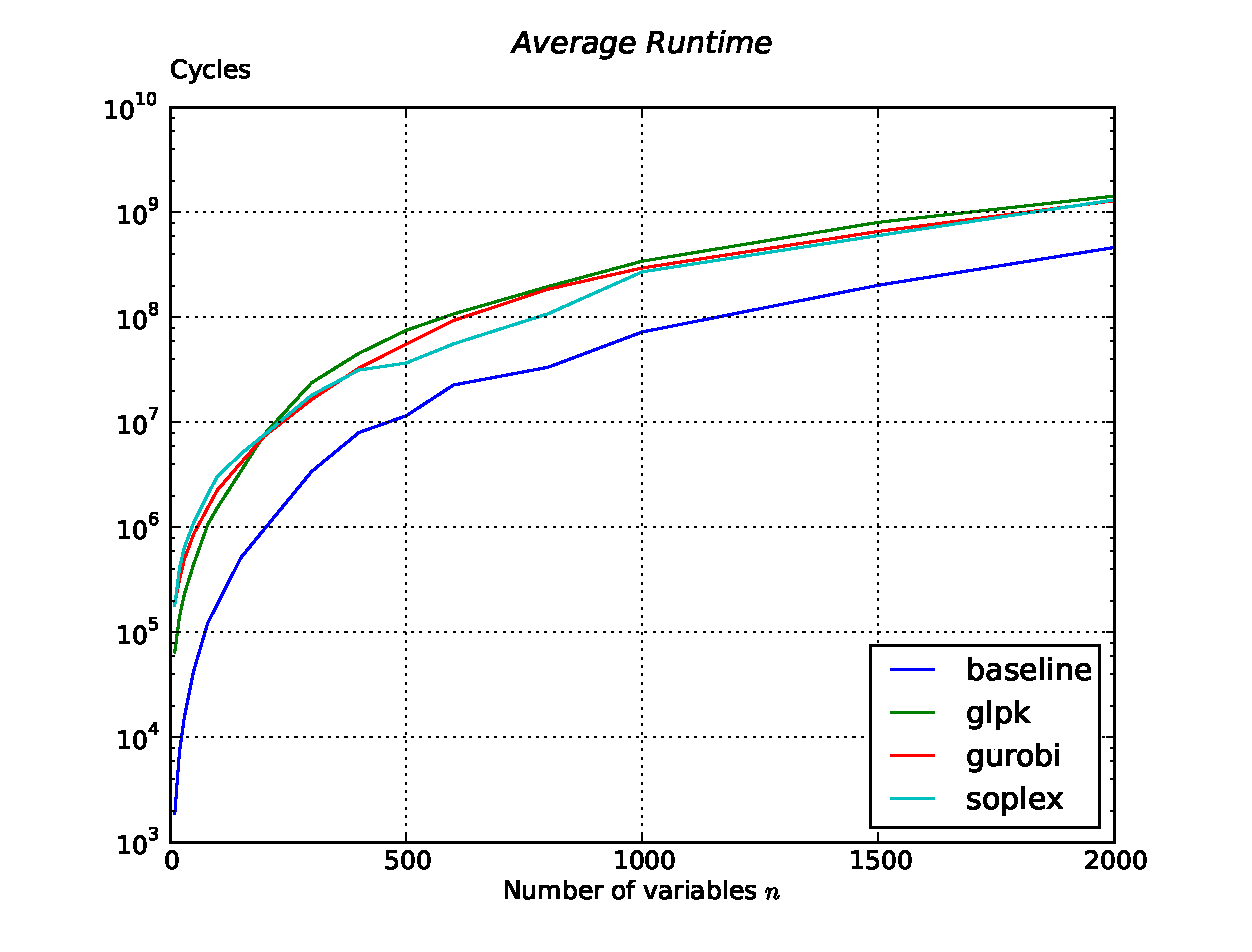
\includegraphics[scale=0.4]{img/results_compare_external.eps}
  \caption{Comparison with Gurobi, SoPlex and GLPK.\label{fig:comp_ext}}
\end{figure}


Profiling of the {\tt swapNxM\_block } implementations showed that between 70\% and 90\% of the time is spent on {\tt \_mm256\_load\_pd } calls.


As shown in Fig.~\ref{fig:res_cachecontrol}, non temporal assignment showed a mostly positive but small effect on the swapping implementations,
while any kind of manual prefetching lead to a considerable slowdown.

\begin{figure}\centering
  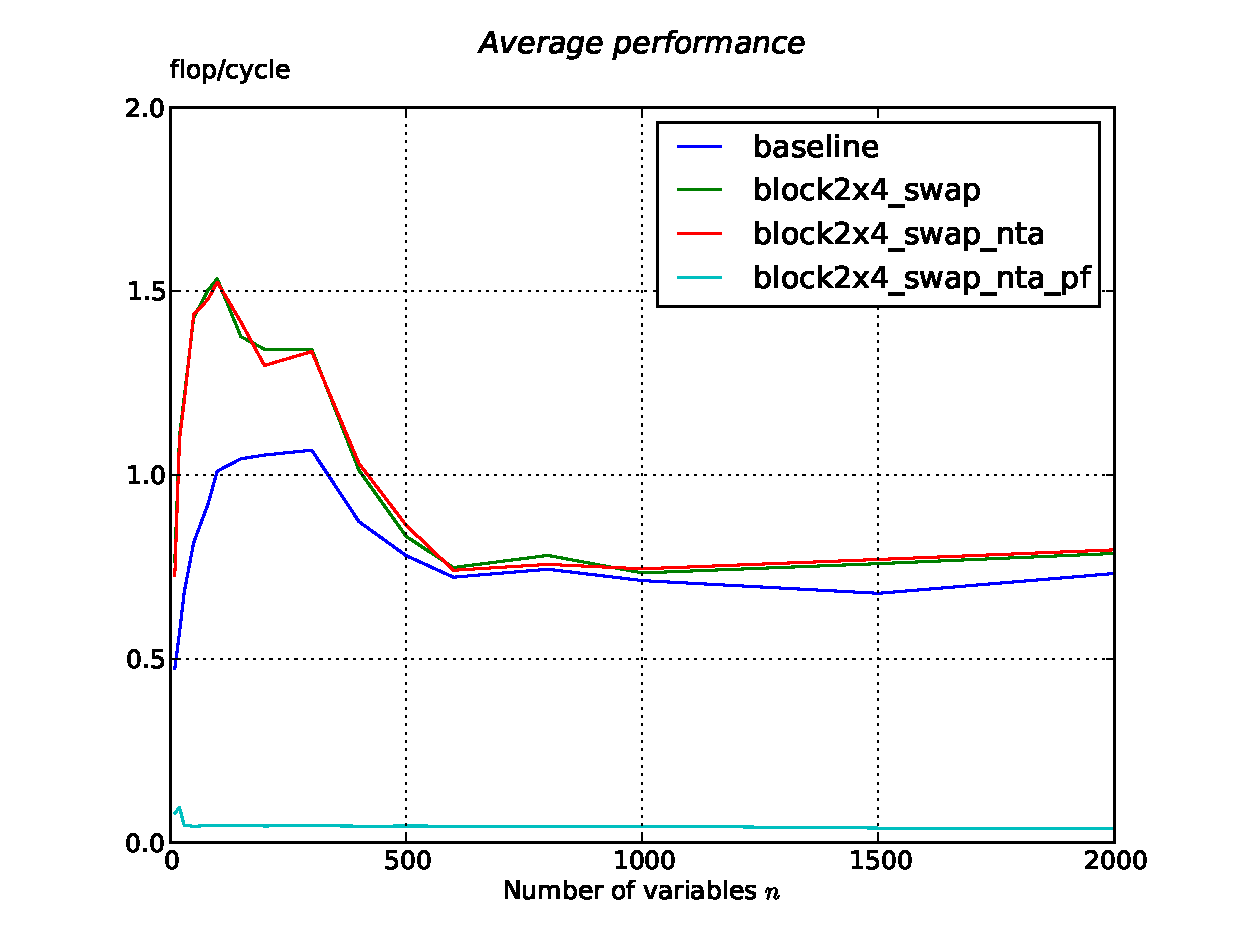
\includegraphics[scale=0.4]{img/results_cachecontrol_novec.eps}
  \caption{Performance of non temporal assignment ({\tt \_nta}) and prefetching ({\tt \_nta\_pf}) implementations of {\tt block2x4\_swap} and the baseline,
  all with the same operation count.\label{fig:res_cachecontrol}}
\end{figure}


From the roofline plot shown in Fig.~\ref{fig:res_roof_high} we learn that our best-performing implementation is very close to the theoretical memory limit.
The corresponding test set starts with problems of size 500 in order to measure only RAM to CPU traffic.

\begin{figure}\centering
  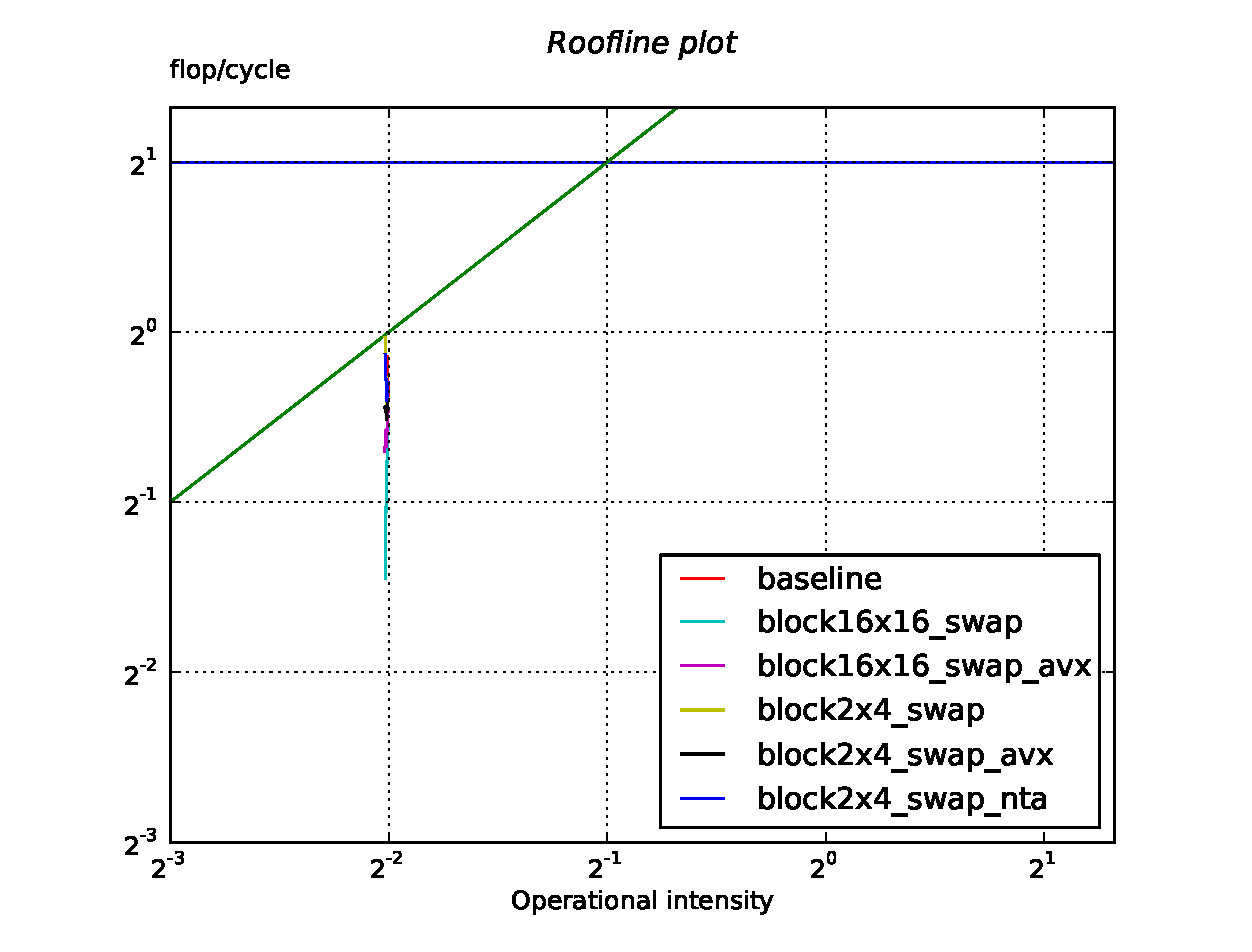
\includegraphics[scale=0.4]{img/roof_high_autovec.eps}
  \caption{Roofline plot, the 8 flop/cycle performance line is cropped away for better readability.\label{fig:res_roof_high}}
\end{figure}



\ptodo{Next divide the experiments into classes, one paragraph for each. In the simplest case you have one plot that has the size on the x-axis and the performance on the y-axis. The plot will contain several lines, one for each relevant code version. Discuss the plot and extract the overall performance gain from baseline to best code. Also state the percentage of peak performance for the best code. Note that the peak may change depending on the situation. For example, if you only do additions it would be 12 Gflop/s
on one core with 3 GHz and SSE and single precision floating point.

Do not put two performance lines into the same plot if the operations count changed significantly (that's apples and oranges). In that case first perform the optimizations that reduce op count and report the runtime gain in a plot. Then continue to optimize the best version and show performance plots.}

\ptodo{{\bf You should}
\begin{itemize}
\item Follow the guide to benchmarking presented in class, in particular
\item very readable, attractive plots (do 1 column, not 2 column plots
for this class), proper readable font size. An example is below (of course you can have a different style),
\item every plot answers a question, which you pose and extract the
answer from the plot in its discussion
\end{itemize}
Every plot should be discussed (what does it show, which statements do
you extract).}

%%%%%%%%%%%%%%%%%%%%%%%%%%%%%%%%%%%%%%%%%%%%%%%%%%%%%%%%%%%%%%%%%%%%%%%%%%%%%%%%
%%%%%%%%%%%%%%%%%%%%%%%%%%%%%%%%%%%%%%%%%%%%%%%%%%%%%%%%%%%%%%%%%%%%%%%%%%%%%%%%

\section{Conclusions}

\ptodo{Here you need to briefly summarize what you did and why this is
important. {\em Do not take the abstract} and put it in the past
tense. Remember, now the reader has (hopefully) read the paper, so it
is a very different situation from the abstract. Try to highlight
important results and say the things you really want to get across
(e.g., the results show that we are within 2x of the optimal performance ... 
Even though we only considered the DFT, our optimization
techniques should be also applicable ....) You can also formulate next
steps if you want. Be brief.}

%%%%%%%%%%%%%%%%%%%%%%%%%%%%%%%%%%%%%%%%%%%%%%%%%%%%%%%%%%%%%%%%%%%%%%%%%%%%%%%%
%%%%%%%%%%%%%%%%%%%%%%%%%%%%%%%%%%%%%%%%%%%%%%%%%%%%%%%%%%%%%%%%%%%%%%%%%%%%%%%%

\section{Further comments}

\ptodo{Here we provide some further tips.

\mypar{Further general guidelines}

\begin{itemize}
\item For short papers, to save space, I use paragraph titles instead of
subsections, as shown in the introduction.

\item It is generally a good idea to break sections into such smaller
units for readability and since it helps you to (visually) structure the story.

\item The above section titles should be adapted to more precisely
reflect what you do.

\item Each section should be started with a very
short summary of what the reader can expect in this section. Nothing
more awkward as when the story starts and one does not know what the
direction is or the goal.

\item Make sure you define every acronym you use, no matter how
convinced you are the reader knows it.

\item Always spell-check before you submit (to me in this case).

\item Be picky. When writing a paper you should always strive for very
high quality. Many people may read it and the quality makes a big difference.
In this class, the quality is part of the grade.

\end{itemize}
}

% References should be produced using the bibtex program from suitable
% BiBTeX files (here: bibl_conf). The IEEEbib.bst bibliography
% style file from IEEE produces unsorted bibliography list.
% -------------------------------------------------------------------------
\bibliographystyle{IEEEbib}
\bibliography{bibl_conf}

\end{document}

